\documentclass[11 pt, twocolumn]{article}

\usepackage{fullpage}
\usepackage{graphicx}
\usepackage{wrapfig}
\usepackage{float}
\usepackage{tikz}
\usepackage{amsmath,amssymb}
\usepackage{empheq}
\usepackage{graphics}
\usepackage{subfig}
\usepackage{float}
%\usepackage{multicol}

\usepackage[english]{babel}
\usepackage[utf8x]{inputenc}
\usepackage{amsmath}
\usepackage{graphicx}
\usepackage{float}
\usepackage[colorinlistoftodos]{todonotes}
\usepackage{amssymb}
\usepackage{amsthm}
\usepackage{mathtools}
\usepackage{color}
\usepackage{enumitem}
\usepackage{upgreek}
\usepackage{listings}  
\usepackage{centernot}

\usepackage[hidelinks]{hyperref}
\usepackage{xcolor}


\usepackage{algorithm}% http://ctan.org/pkg/algorithm
\usepackage{algpseudocode}% http://ctan.org/pkg/algorithmicx
%\usepackage[margin=1.05in]{geometry}
\usepackage[a4paper, total={6.75in, 10.45in}]{geometry}
\usepackage[parfill]{parskip}
\DeclarePairedDelimiter{\ceil}{\lceil}{\rceil}
\setcounter{secnumdepth}{0}

\title{Comparing Protein Secondary Structure Prediction Using Hidden Markov Models and Conditional Random Fields}
\author{Tahmid Rahman and Muha Haque}

\begin{document}
\maketitle

\begin{abstract}
The tertiary and quaternary structures of proteins are vital to determining both their stability and how they interact with other proteins. Predicting these structures from a protein's primary structure is a difficult problem; however, the problem becomes more tractable when using secondary structures to predict tertiary structures, and using tertiary structures to predict quaternary structures. As such, being able to confidently predict secondary structures using primary structures is an important intermediate step. Towards this end, we compare two models for predicting protein secondary structures given the primary structures: Hidden Markov Models (HMMs) and Conditional Random Fields (CRFs). We randomly sample from a list of 1975 proteins for which the secondary structures have been identified to construct training sets of various sizes and testing sets of 200 proteins. Our results reveal that because our models for HMMs and CRFs are fairly simple, large training set sizes cause their predictions to converge to whichever secondary structure is most abundant in the training data.  
\end{abstract}

\section{Introduction}

Obtaining deep knowledge of protein structures is an important step in understanding various biological mechanisms and for creating drugs that can activate or inhibit different proteins, among many other applications. This is because the three-dimensional structure of a protein largely determines its function. This link between a protein’s structure and its function combined with recent advances in high throughput sequencing that allows us to know 1000 times as many sequences as we do structures stresses the need for accurately predicting protein structures \cite{Dill}. 

It is difficult to use a protein's sequence of amino acids, the primary structure, to predict its three-dimensional folding, the tertiary or quaternary structures. It is much easier, however, to incrementally work up and use the primary structure to predict the secondary structure, the secondary structure to predict the tertiary structure, and so forth. In this paper, we focus on the first of these intermediate steps. The secondary structures of proteins are a result of hydrogen bonding between amino acids on the protein chain can be classified into three specific substructures: $\alpha$ helices, $\beta$ pleated sheets, and coils. The interactions between these three types of secondary structures informs the three dimensional folding. Figure \ref{fig:proteinStructure} offers a visual example of the different types of protein structures.

\begin{figure}
\centering
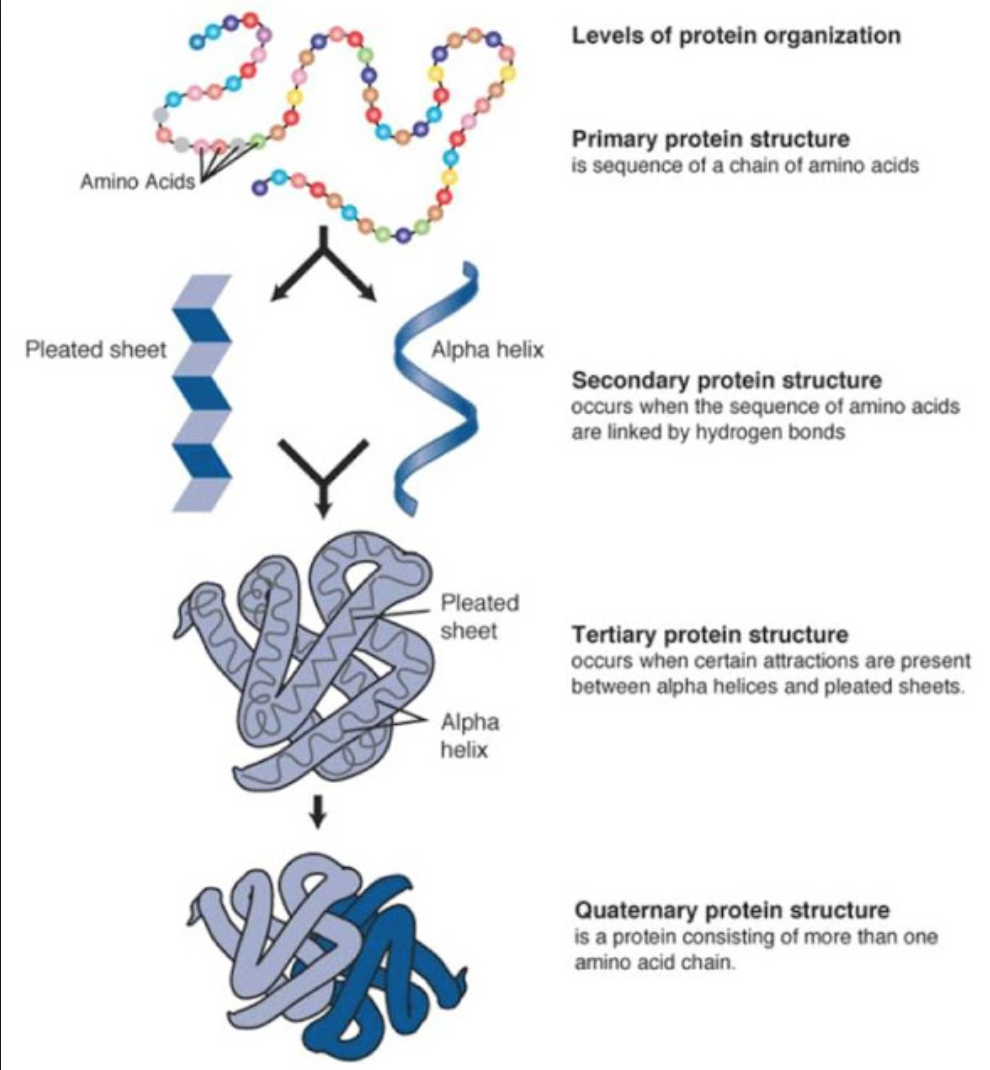
\includegraphics[width = .4\textwidth]{StructuresOfProteins.png}
\caption{This figure illustrates the different types of structures of a protein, ranging from primary to quaternary. We place special emphasis on understanding the tertiary structures of proteins. Image from:\url{http://www.majordifferences.com/2013/02/difference-between-primary-and.html\#.WQMxdVKZNE4}}
\label{fig:proteinStructure}
\end{figure}

Many different models, and combinations thereof, have been applied to predict protein secondary structures. The problem statement itself can vary. The question we tackled can be identified as a classic example of a supervised learning problem. Our input is a set of primary structures for many different proteins. The labels are a corresponding set of secondary structure sequences, one such sequence per protein. There is a one to one mapping between the amino acids of a protein and the secondary structure to which the amino acids belong. Our problem is to train a model that accurately predicts the secondary structures when given only the amino acid sequence as input. For this supervised learning task, we compared two types of models that have proved useful in sequence tagging: HMMs and CRFs. 

We vary the amount of supervised training data given to each of the two models as our main parameter. Per training data size, we assess the accuracy of the models’ predictions. The typical curve when pitting accuracy against training data size is one that is concave down; increasing the number of training examples yields diminishing returns until the model begins overfitting, after which the model's accuracy with proper test sets take a hit due to its inability to generalize well. Contrary to expectation, our accuracy versus training set size curves are concave up. Furthermore, using lots of training data caused our HMM and CRF to converge to predicting everything as a helix.  This highlighted the importance of not using overly simple models for protein secondary structure prediction, as was the case since we used HMMs and CRFs out of the box. 

\begin{figure}
\centering
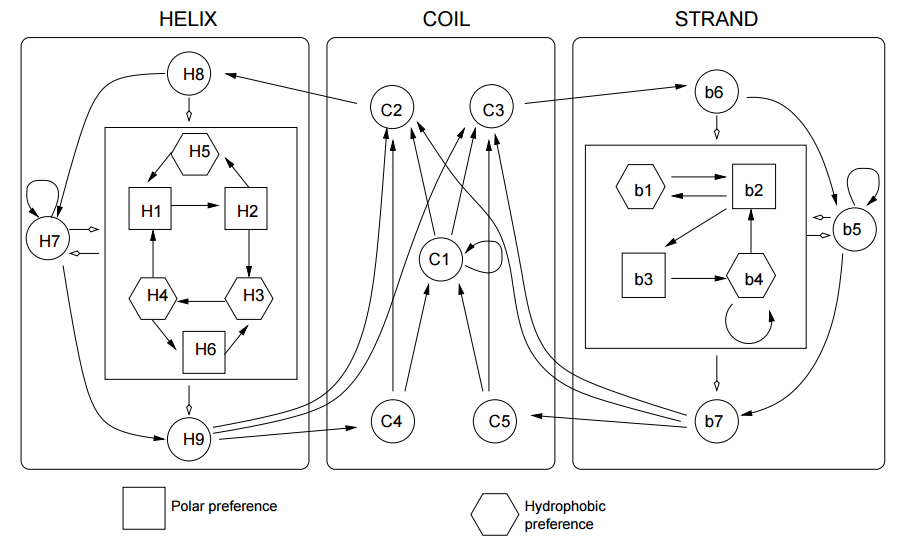
\includegraphics[width = .4\textwidth]{ComplexHMMModel.png}
\caption{The figure above comes from this study \cite{Martin} by Martin et. al and demonstrates a 21-state model for HMMs that they use for their experiments, with each of the possible secondary structures showing multiple states and dependencies between them.}
\label{fig:compHMMMod}
\end{figure}

\section{Related Works}

%http://citeseerx.ist.psu.edu/viewdoc/download?doi=10.1.1.105.2294&rep=rep1&type=pdf
%also, if we can't find citation for the link above, this one is by the same people and pretty similar: http://ieeexplore.ieee.org/document/1556511/?reload=true
The models we present in this paper cannot compare to ones trained in other studies. Martin et.al\cite{Martin} researched and experimented with complex HMM models that could be used for protein secondary prediction. Their experiments used 2530 sequences, with fourfold cross-validation performed on 2024 randomly selected sequences and the remaining 506 sequences acting as an independent test set. They acknowledge that the simplest model that can be used is a three-state model such as the one we use, where the three states are the three possible secondary structure classes: helices,
sheets, and coils. They found that such a model had a correct prediction rate of approximately 58.3\%. To improve upon this score, they replaced the simple emission models traditionally found in HMMs with handcrafted Markov models tailored for each of the three secondary structures. For helices and sheets, this allowed them to integrate information about frequently represented amino acid sequences and their secondary structures. Their models also noted states that showed preference for polar or hydrophobic amino acids. The resulting overall HMM had 9 states for the helix section, 7 states for the sheet section, and 5 states for the coil section, for a total of 21 states. It had a prediction accuracy of approximately 72\%\cite{Martin}. This complex model shows how HMMs with more states can account for the biological interactions that arise in the protein secondary structure, and can be seen in Figure \ref{fig:compHMMMod}. 



CRFs have also been used successfully to predict protein secondary structures. Lukov et.al\cite{Lukov} used CRFs to create a model for the secondary structure prediction problem that held a competitive edge against 28 other methods that were state of the art at that time. In particular, their research focused on Integral Membrane Proteins (IMPs), for which the location of helices is especially important. As one of the first studies to use CRFs in the field of bioinformatics, Lukov et.al were particularly interested in the ability to integrate multiple features and dependencies between them. These features include the 20 basic amino acids, like we use in our model, as well as start, end, and edge features, features focusing on hydrophobic and hydrophilic qualities, neighboring features, electrical and chemical features, etc. In total, their CRF model extracted 18 features from the protein primary structure in order to predict the secondary structure. When the model was tested against the benchmarks for transmembrane helices prediction, it was 84\% accurate using amino acids. This CRF model was also successful in analyzing a protein complex called cytochrome c oxidase. The model found success by considering many combinations of features and allowing for a more complex, biological model, as shown in Figure \ref{fig:compCRFMod}.

\begin{figure}
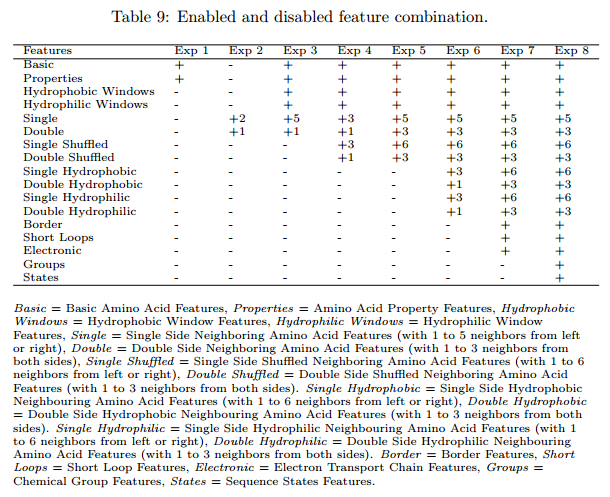
\includegraphics[width = .5\textwidth]{ComplexCRFMod.png}
\caption{Lukov et. al \cite{Lukov} use CRFs to account for various combinations of potential features of the input amino acid sequences, as shown above, to allow them to predict the secondary structures.}
\label{fig:compCRFMod}
\end{figure}

\section{Models}

In this section, we unravel the details of HMMs and CRFs, the two models we used to predict protein secondary structures. Each of these models underwent supervised training using data sets of various sizes. The models learned differently depending on whether the algorithms were generative, as is the case for HMMs, or discriminative, as is the case for CRFs. 

\subsection{HMMs}
Hidden Markov Models utilize Markov chains with both observed data, called symbols, and hidden data, called states. HMMs are generative models, modeling the likelihood of seeing the data given the hidden model using joint distributions. This means that observations are independent of other observations within labels. The goal of HMMs is to estimate $p(x, y)$, where $x$ is a sequence of symbols, or emissions, and $y$ is a path through the states. HMMs can be modeled as follows \cite{Lukov}:
$$ p(x,y) = p(y_1)p(x_1\mid y_1) \prod_{i=2}^{n} p(y_i \mid y_{i-1}, x_i)$$

There are three main algorithms that HMMs use: the forward algorithm, the Viterbi algorithm, and the forward-backward, or Baum-Welch, algorithm. The forward algorithm allows us to determine $p(x)$, the probability of encountering a sequence $x$. The Viterbi algorithm finds the most likely path for a sequence. Finally, we need to learn the HMM parameters, which can be done using the forward-backward algorithm, or the Baum-Welch algorithm. The goal in this last step is to maximize the likelihood of the model, or find $\text{argmax} P(x\mid \theta$) such that $\theta = {a_{lk}, e_k(i)}$, where $a_{lk}$ represents the transition between states $l$ and $k$ and $e_k(i)$ represents the emission value. Then, expectation-maximization is repeated on these parameters until convergence. Due to the supervised nature of our training process with the HMM, we can estimate the parameters by counting the number of times each parameter is used across the training set.

HMMs can also be modified to utilize higher-order Markov chains. The following is a $k$th order Markov chain assumption: 
$$P(x_i \mid x_{i-1} , ... x_1) = P(x_i \mid x_{i-1},...x_{i-k})$$ 
This allows us to consider relationships between
$k$ states, rather than just immediate states in a 1st-order model. Because the implementation we used, the NLTK package, did not allow us to test higher orders, it is worth noting that our model's predictive ability is more simplistic as a result.

\begin{figure}
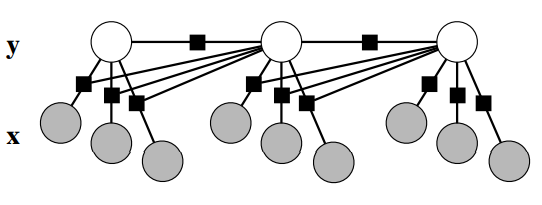
\includegraphics[width = .5\textwidth]{LinearChainCRFGraph.png}
\caption{The figure above shows the graphical model of linear-chain CRFs. Here, $x$ is a vector of observation features, and $y$ is the tag associated to $x$.}
\label{fig:linearchainCRFGraph}
\end{figure}

\subsection{CRFs}
Conditional random fields are the other model we used to predict protein secondary structures. CRFs are conditional distributions $p(y|x)$ and, as such, the model can better account for interactions
between features of the input. Graphically, the underlying model of CRFs is an undirected chain \cite{Sutton}, as shown in Figure \ref{fig:linearchainCRFGraph}. Because they use conditional distributions instead of joint distributions like HMMs, which are generative models,
CRFs are described as discriminative models. Generative models need to make assumptions about how the observations are generated from the labels whereas discriminative models are able to directly model this\cite{Lukov}. This difference is due to the fact that a model
of $p(x)$, which often struggles to represent complex dependencies between features of the input, is not needed for discriminative models \cite{Sutton}. 

A more thorough explanation of the theory behind CRFs can be found in \cite{Sutton}. We focus specifically on linear-chain CRFs, because that particular model is utilized by the CRF implementation we use, MALLET.  The first step to understanding linear-chain CRFs is to first understand feature functions. Feature functions are real-valued functions of the form $f_k(y_t, y_{t-1}, x_t)$, taking in the current and previous tags, denoted $y_t$ and  $y_{t-1}$, and the current observation in the sequence, $x_t$.  These feature functions are then assigned weights , $\lambda_k$, that are learned. Each transition between states $i$ and $j$ can be represented as $f_{ij}(y, y\prime, x)) = 1_{y=i}1_{y\prime=j}$, and each state-observation pair $(i,o)$ as 
$f_{io}(y, y\prime, x)) = 1_{y=i}1_{x=o}$, where $1_{\text{condition}}$ is an indicator variable that outputs $1$ when the condition is met. Recall the mathematical model for HMMs and note that we can substitute feature functions in via $p(y,x)$ and use that for $p(y|x)$ to we get a mathematical model for linear chain CRFs.  To obtain the conditional distribution $p(y|x)$, we first express the traditional joint distribution used for HMMs, $p(y,x)$, as:

$$p(y,x) = \frac{1}{Z}\text{exp}\{\sum_{k=1}^{K}\lambda_k f_k (y_t, y_{t-1}, x_t)\}$$

where $Z$ is a normalization factor.

We can work from the above generalization of the mathematical model for HMMs to derive:

$$p(y|x) = \frac{1}{Z(x)}\text{exp}\{\sum_{k=1}^{K}\lambda_k f_k (y_t, y_{t-1}, x_t)\}$$

where $Z(x)$ is an instance specific  normalization function.

In this way, linear-chain CRFs can be understood relative to HMMs\cite{Sutton}. Specifically,  HMMs can be thought of as a weaker version of linear-chain CRFs. 

Parameter estimation for linear-chain CRFs is often performed by penalized maximum likelihood, specifically the conditional log likelihood in this case. Additionally, regularization, a penalty on weight vectors with large norms, can be used to handle the large number of parameters and avoid overfitting. In terms of inference, the forward, backward, and Viterbi algorithms can be used fairly similarly to their use for HMMs, with the difference being that they are used to compute $Z(x)$ rather than $p(x)$.

Like with higher order HMMs, higher order linear-chain CRF models should represent complex data with interactions between features more accurately. Specifically, higher order CRF models can also take into account interactions between nearby features, i.e. those separated by features between them, rather than being limited just to neighboring features. Because MALLET allows us to manipulate the order of the CRF model we chose to use, we were interested in seeing whether this strength of higher-order models could account for complex elements of our training data, such as the tendency of nearby helices to interact with each other, and have a more intricate predictive model as a result.

Furthermore, CRFs are generally a stronger tool than HMMs. For one, it's possible to define a much larger set of features to use for CRFs, as  Lukov et. al demonstrated \cite{Lukov}. For another, the weights that a CRF learns are not probabilities, meaning that they are less restricted.

\section{Experiments}

Having given details of the two models at play, we now discuss the details of our experimental methodology, our results, and provide an analysis of our results. For HMMs, we used the NLTK package and for CRFs, we used MALLET. We first trained HMMs and CRFs using randomly sampled training sets of various sizes to see how sensitive to overfitting or underfitting these models were. We then tested these models in their ability to correctly predict secondary structures using a randomly sampled test set. 

\subsection{Experimental Methodology}

\begin{figure}
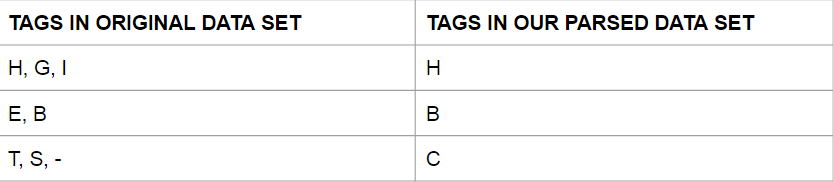
\includegraphics[width = .4\textwidth]{MappingOfTags.png}
\caption{In parsing our list of proteins from an external database\cite{Zhang}, we simplified the number of secondary substructures by mapping them as shown in the figure above to H for alpha helices, B for beta sheets, and C for coils.}
\label{fig:MapTags}
\end{figure}


\begin{figure*}[!ht]
\begin{tabular}{ccc}
\subfloat[HMM]{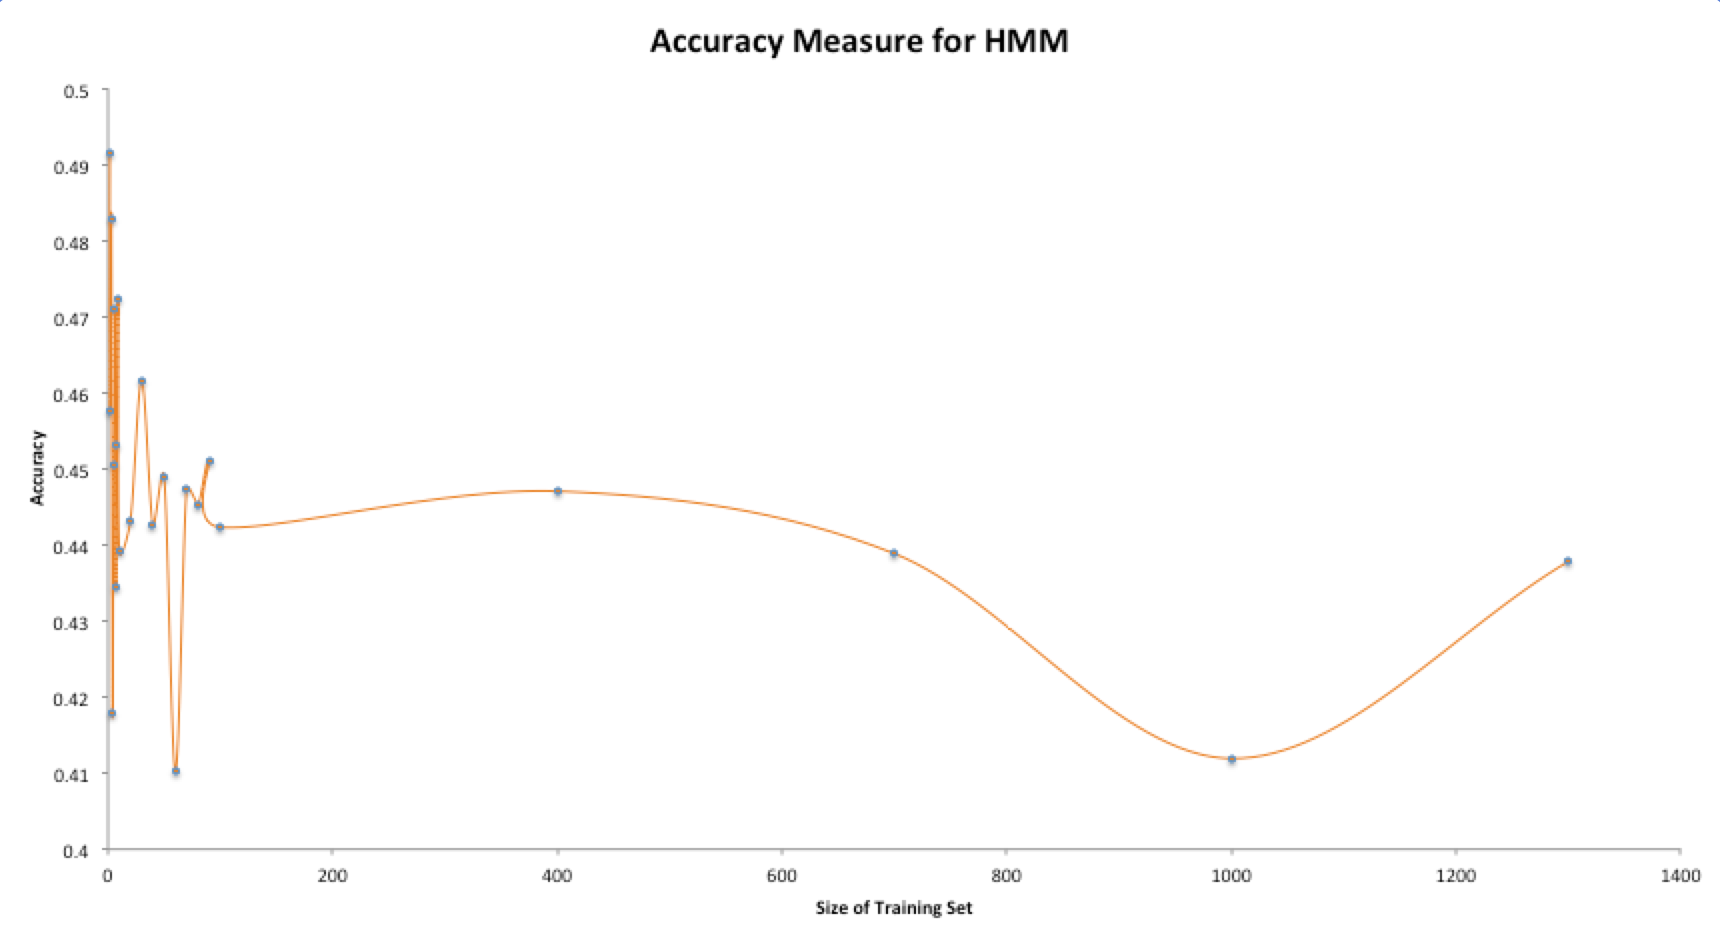
\includegraphics[width = .3\textwidth]{HMMData.png}} &
\subfloat[CRF Order 1]{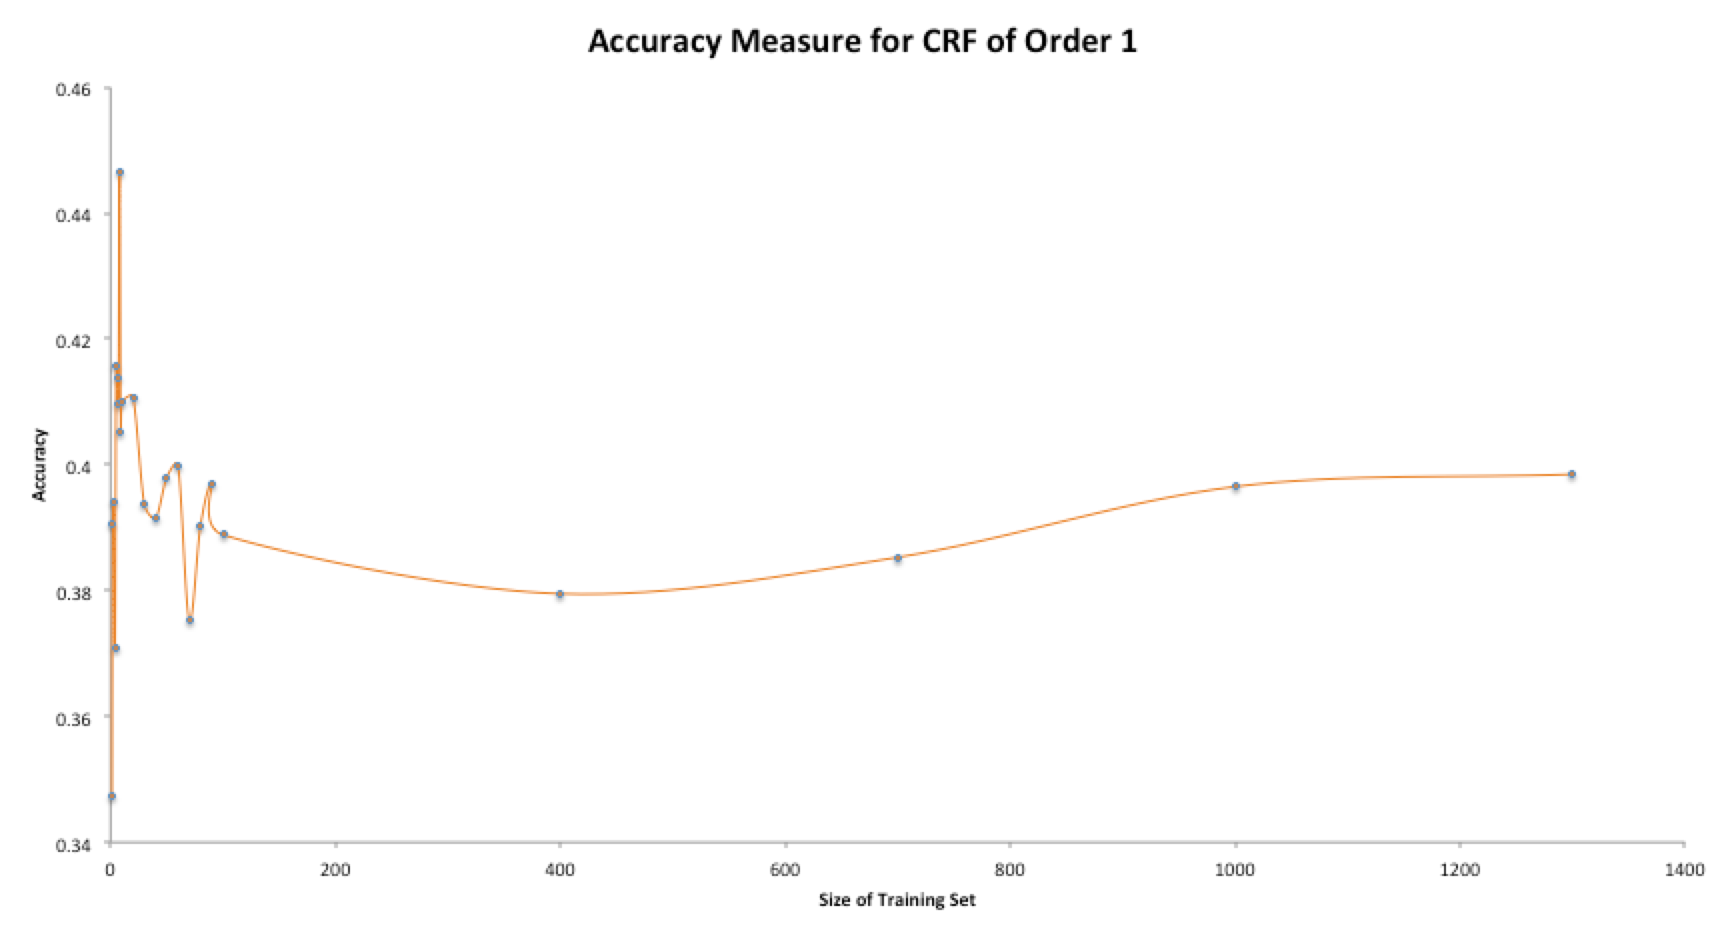
\includegraphics[width = .3\textwidth]{CRFOrder1Data.png}} &
\subfloat[CRF Order 3]{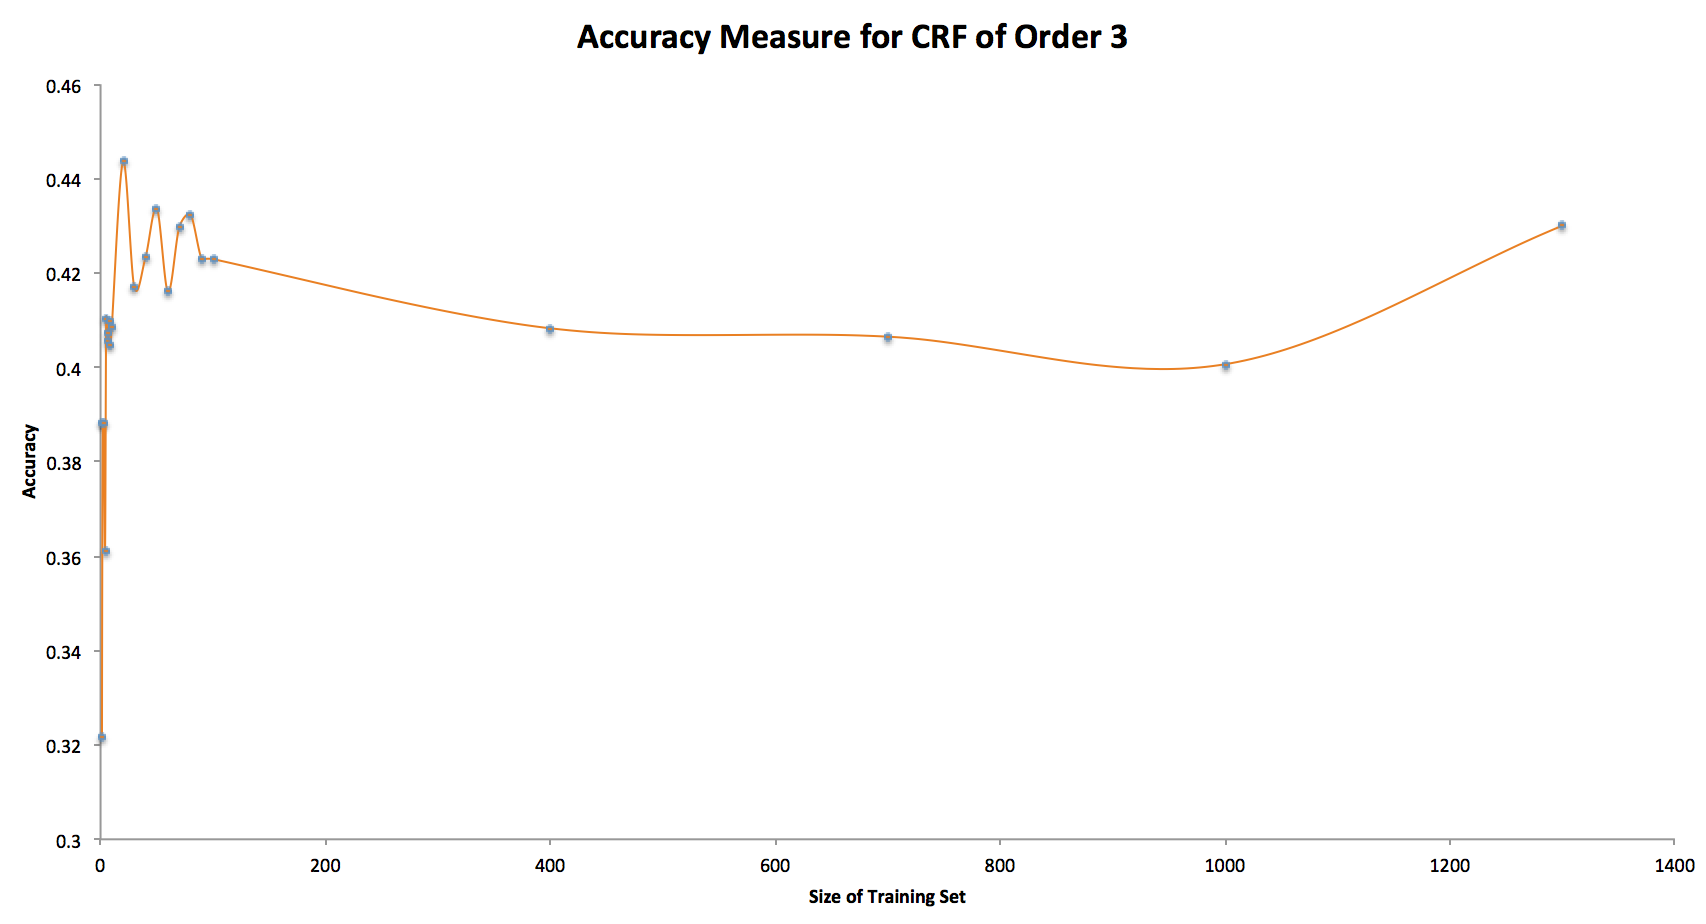
\includegraphics[width = .3\textwidth]{CRFOrder3Data.png}} \\
\end{tabular}
\caption{These figures chart the accuracy of the predictions made by HMMs and CRFs against the sizes of the training set. In all cases, the accuracy score is a measure of the number of correctly tagged test examples over the total number of test examples. In other words, it is the percentage of correctly tagged test examples. The first order CRF and the HMM had high accuracy values when trained with ten or fewer examples. The third order CRF had a similar behavior, but the dip in accuracy as training sizes increased was less extreme.}
\label{fig:dataFigure}
\end{figure*}

The main parameter we vary in our experiments is the size of the training set given to each of our models.
Specifically, the training  input sizes range from 1 to 10 in increments of 1, 10 to 100 in increments of 10, and 100 to 1300 in increments of 300. We also train 1st and 3rd order CRF models for each of our training sizes. For each set of conditions given a model, we train and test three times. Our final accuracy scores are an average of the three. 

To construct our training sets, we randomly sampled from a list of 1975 proteins for which secondary structures have already been identified.  We obtained this list of proteins from  a database kept by the University of Alberta\cite{Zhang}. The original database differentiated between different types of helices, sheets, and coils. We simplified the data by converting the a plethora of labels for different types of secondary structures into one of three, more general labels. The conversion map can be seen in Figure \ref{fig:MapTags}. 

For our test sets, we randomly sampled 200 protein sequences and their corresponding secondary structures. For our training sets, we randomly sampled however many proteins as our training input size parameter dictated. 


We fed each protein sequence from our test set into our two models after training them. The models would then tag the sequences with predicted secondary structures. For each of the three possible tags, $\alpha$ helices, $\beta$ sheets, and coils, we counted the number of  true positives, false positives, true negatives, and false negatives . Using these measures instead of a simple overall count of accuracy gave us a better sense of  the sources of error; for example, having very high counts for true positives and false positives for a specific tag reveals that the model is guessing  almost everything as that tag.



\subsection{Results}

Our results indicated that increasing the sizes of the training input across all models either had little to no benefit or actively harmed the models' ability to accurately predict the secondary structure. When comparing accuracy scores (the ratio of the total number of correct predictions to the total number of predictions made), CRFs performed better than HMMs. However, the different orders of the CRFs did not make a noticeable difference. These results can be observed in Figure \ref{fig:dataFigure}.

\begin{figure}
\centering
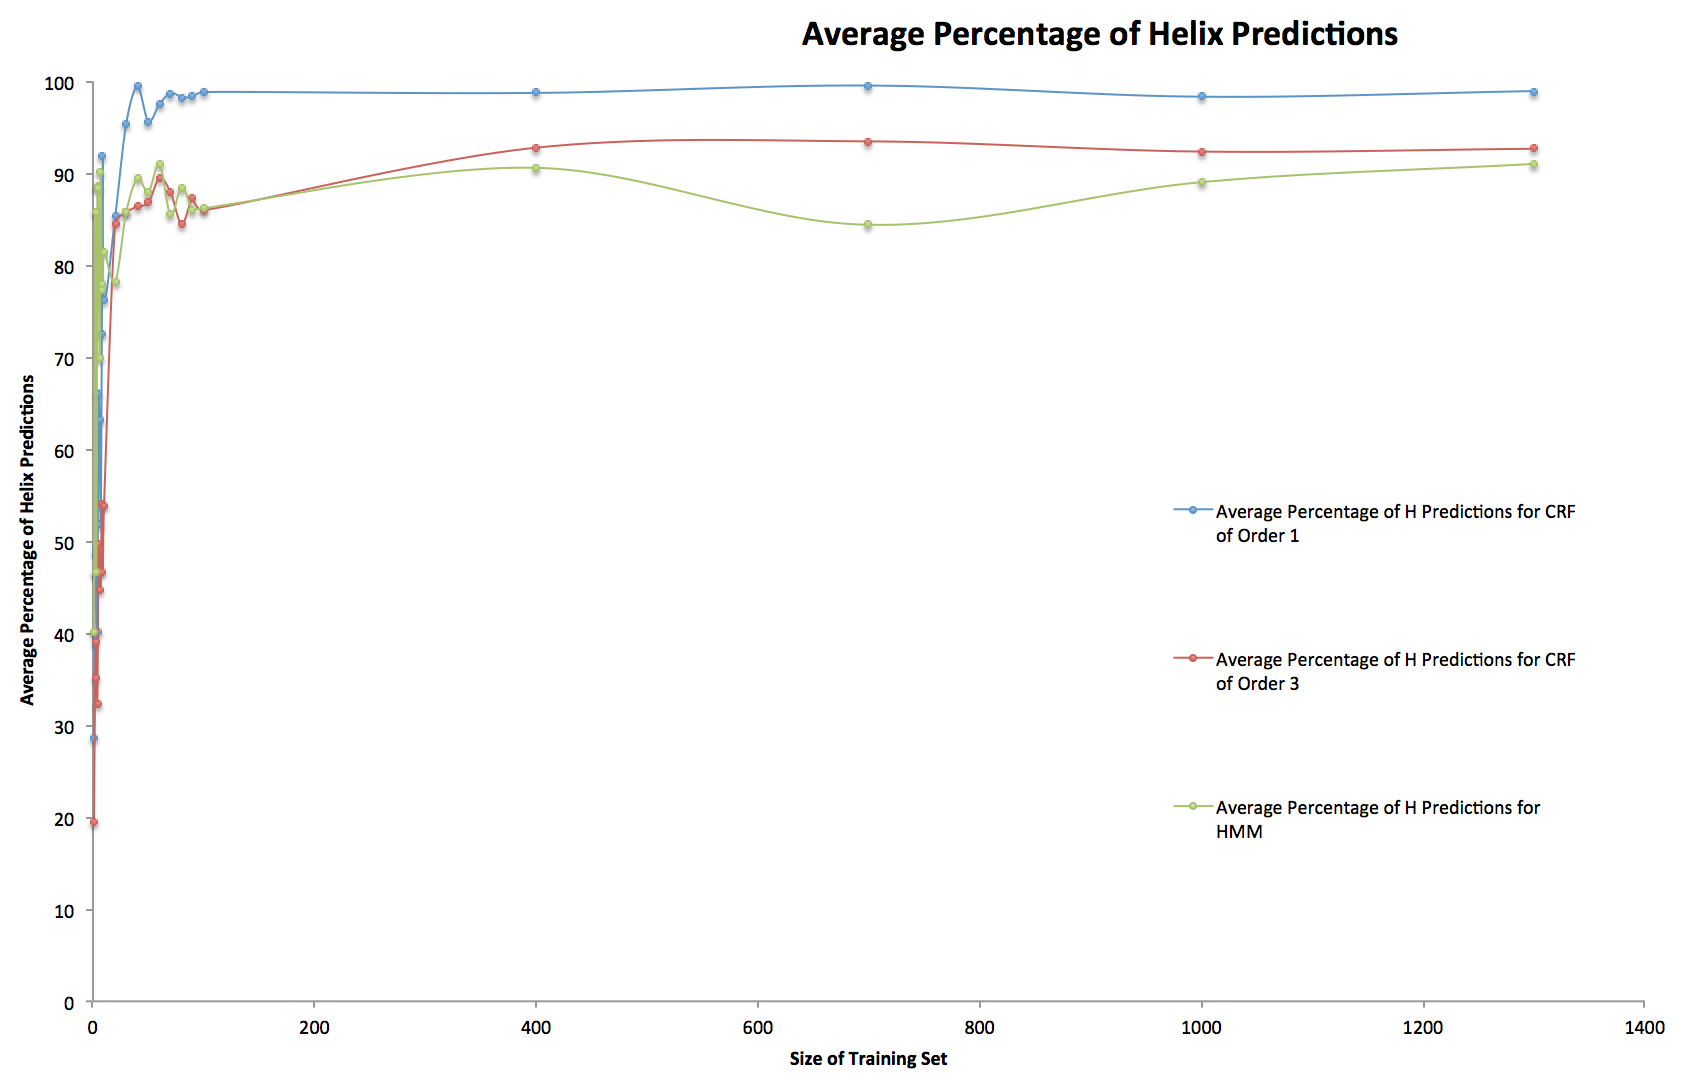
\includegraphics[width = .5\textwidth]{Helix_Predictions.png}
\caption{The above graph compares the percentage of predictions output as a helix against the number of sequences used for the training set. It shows that for large training sets, the CRFs and the HMM we trained will predict the secondary structure to be a helix almost all the time.}
\label{fig:helixPred}
\end{figure}

By measuring the true positive and false positive counts for each of the three possible tags, we also enabled ourselves to observe the main sources of error for these models. For  HMMs and CRFs, large training  sets led to the model learning  to predict  the secondary structure as a helix close to one hundred percent of the time. This can be observed  in Figure \ref{fig:helixPred}. 

\subsection{Discussion}

The curves mapping accuracy against training set size are all concave up. That the accuracy for the largest training set sizes  matched the accuracy for small training set sizes does not tell the full story, however. Using the model out of the box and training it the way we did made it hypersensitive to overfitting. The amino acid sequences in our data set contained more helices, but only by a relatively small amount. As such, larger numbers of training examples caused our model predictions to converge towards predicting every secondary structure as a helix. The more these models predicted a helix, the less accurate their predictions became. This continued until almost all, if not all, the predictions were helices. Once this point was reached, the accuracies increased slightly because helices were slightly more abundant than any other type of secondary structure. 


We did attempt to train the HMM by culling examples that contained helices in its secondary structure more than a third of the time from our training sets of sizes larger than 100. However, this led our HMM to predict beta sheets almost all the time. When culling a second time to remove examples that contained $\beta$ sheets in its secondary structure more than a third of the time, our HMM learned to predict coils almost all of the time.

There are several reasons to explain this source of error. First, our three-state HMM might be too simple. Similarly, using CRFs out of the box without adding more complex structures might have also been too simple. Second, we may have not constructed our training sets to consist of examples that would best help with the learning process and avoid both overfitting and underfitting. Our HMM took as input single amino acids and only looked at the previous character to output a prediction as it was a first order model. Meanwhile, we gave CRFs windows of fifteen amino acids to learn from. Our features in both cases were the amino acids. This may not have been the best features to give to an HMM or CRF. Perhaps interpreting the sequence of amino acids a different way could have yielded more a higher accuracy score and a lower likelihood of converging to a specific secondary structure as the ultimate prediction. Third, our data set itself might have had enough errors and noise that there wasn't much of a biological connection between primary and secondary structures to learn. 

\section{Conclusion}

When comparing  HMMs against CRFs on  their ability to accurately predict protein secondary structures, our results suggest  that there is not much discrepancy. However, these results are not conclusive; the means with which we  wired up the data to train HMMs and CRFs were  basic. Furthermore, though the accuracy scores were not significantly worse  when given many hundreds or even a thousand training examples over just ten or twenty, the actual predictions easily converged to just one tag, the helix, when provided too large a training set. 

An interesting problem we have thus come across is that contrary to what one may think about HMMs, large amounts of training data can hurt the model. A query that arises naturally from this observation is determining the least complex Markov Model  for predicting secondary structures that doesn't overfit  to the data and converge to just one tag after given a relatively small number of training examples. 

One way to begin constructing such a model would be to use the approach suggested by Martin et. al \cite{Martin}. Their approach takes into account some of the deeper biological characteristics of the input as well as models the relationships between them. An example of this is mapped out in Figure \ref{fig:compHMMMod}. Within helices, for example, Martin et. al identified the amphiphilic nature of helices and used this as a basis to incorporate polar and hydrophobic states into their helix model \cite{Martin}. To get more accurate prediction results in the future, we could benefit from domain knowledge which could indicate what other states we could add to our HMM.

Additionally, Martin et. al had data that was more thoroughly parsed before learning than in our model. Although they did randomly select the 2024 sequences that would not be part of the independent training set, they performed four-fold cross validation on this set of sequences; only 75\% is used for parameter estimation and the rest are used to test. Furthermore, their secondary structure definition used a laboratory-designed method called the STRIDE Method that may have also made their input data more conducive to learning than ours\cite{Martin}. Although we did attempt to cull our examples, as mentioned in the Discussion, perhaps in future studies we could perform more rigorous analysis on our data to set to make it more suitable for our HMM model to train on and learn from.

As for CRF's, we could similarly benefit from using domain knowledge more and incorporating more features into our model, as did Lukov et. al \cite{Lukov}. Our model only briefly takes advantage of how CRF's are less bound and more open to complex input dependencies than HMM's; this is when we test with a higher-order model. Although that particular test did not yield significantly better results, perhaps incorporating more biological features into how we represent our input could also allow higher-order CRF models to be more effective.

In summary, we learned that simple learning models were not sufficient for data as complex as ours. The implementations are limited in terms of how they can learn input, particularly the NLTK package's lack of a higher-order HMM model. In future studies, we can compensate by providing them with input that acknowledges more biological features and complexities. By giving our models more complex, but realistic, representations of the primary protein structures, they can do a better job of learning the training data and have a stronger performance when tasked with secondary structure prediction.
\begin{thebibliography}{1}

\bibitem{Dill}
Dill, K.A., and McCallum, J.L. "The protein-folding problem, 50 years on." Science 338 (2012): 1042-1046.

\bibitem{Lukov}
Lukov, L., Chawla, S., Liu, W., Church, B., Pandey, G.. "Protein Secondary Structure Prediction with
Conditional Random Fields." Technical report / University of Sydney. School of Information Technologies 650 (2010): 1-28.

\bibitem{Martin}
Martin, J., Gibrat, J., and Rodolphe, F.. "Hidden Markov Model for protein secondary
structure." International Symposium on Applied Stochastic Models and Data Analysis (2005): 180-187

\bibitem{Sutton}
Sutton, C., and McCallum, A.. "An Introduction to Conditional Random Fields for Relational Learning." Foundations and Trends® in Machine Learning 4.4 (2012): 267-373.

\bibitem{Zhang}
Zhang H, Zhang T, Chen K, Kedarisetti KD, Mizianty MJ, Bao Q, Stach W, Kurgan LA. "Critical Assessment of High-throughput Standalone Methods for Secondary Structure Prediction." Briefings in Bioinformatics (2011).
\end{thebibliography}




\end{document}